\section{Heur\'istica Golosa}
\subsection{Explicacion detallada de la heur\'istica propuesta}

La heur\'istica desarrollada consiste en una modificaci\'on del algoritmo de camino m\'inimo de Dijkstra.

\subsubsection{Inicializaci\'on}

En la etapa de inicializaci\'on se declaran cuatro vectores a utilizar:

\begin{enumerate}

\item CostosW2
\item Predecesores
\item CostoRecorrido
\item CostosW1
\end{enumerate}

CostosW2, es an\'alogo al vector distancias del algoritmo de Dijkstra, siendo $w_2$ la distancia a minimizar, guarda el costo $w_2$ del camino provisorio para cada nodo que va armando el algoritmo. Predecesores es an\'alogo al vector predecesores de dicho algoritmo, indicando para cada nodo cu\'al es su predecesor en su camino, mientras que CostoRecorrido almacena el costo $w_1$ del camino recorrido.

\vspace{2mm}

CostosW1 almacena el costo $w_1$ del camino m\'inimo de cada nodo hasta el nodo de llegada, por razones que explicamos a continuaci\'on:

\vspace{2mm}

Luego de la declaraci\'on de los vectores, se calculan los caminos m\'inimos en cuanto a costo $w_1$ de todos los nodos hacia el nodo de llegada. Ya que el grafo es simple, las aristas no tienen orientaci\'on definida, por lo cual dados dos nodos $v_1$ y $v_2$, el camino m\'inimo de $v_1$ a $v_2$ es igual al camino m\'inimo de $v_2$ a $v_1$. Esto nos permite ejecutar una \'unica vez el algoritmo de Dikjstra desde el nodo de llegada hasta todos los dem\'as sobre $w_1$ y obtener lo buscado.

\vspace{2mm}

Una vez obtenidos los caminos m\'inimos de cada nodo a la llegada en cuanto a costo $w_1$, \'estos nos permiten conocer lo siguiente:

\begin{enumerate}
\item Al iniciar el algoritmo, aquellos nodos para las cuales no existe un camino de longitud $w_1 \leq K$ hasta el nodo llegada, los cuales nuestro algoritmo va a ignorar.
\item En medio de la ejecuci\'on del algoritmo, desde un nodo $v$ podemos saber si el nodo $x$ de la pro\'oxima arista $(v,x$ a considerar tiene al menos un camino $c$ hasta el nodo llegada tal que, el costo del camino formado por la uni\'on de $c$ ($costoW1(x)$) y el recorrido hasta ahora ($costoRecorrido(v)$) es $\leq K$. En caso de no tenerlo, desde ese nodo no hay un camino v\'alido hasta la llegada, por lo tanto nuestro algoritmo va a descartar esta arista por otra que tenga al menos un camino posible hasta la llegada. Esto lo podemos conocer, ya que la ejecuci\'on de Dijkstra inicial nos brinda el costo $w_1$ del camino m\'inimo desde el nodo $x$ hasta la llegada, por lo tanto  si $costoRecorrido(v)$ + $costo(v,x)$ + $Costosw_1(x)$ $\leq$ $K$ sabemos que existe al menos este camino v\'alido, caso contrario descartamos la arista.
\end{enumerate}

\begin{center}
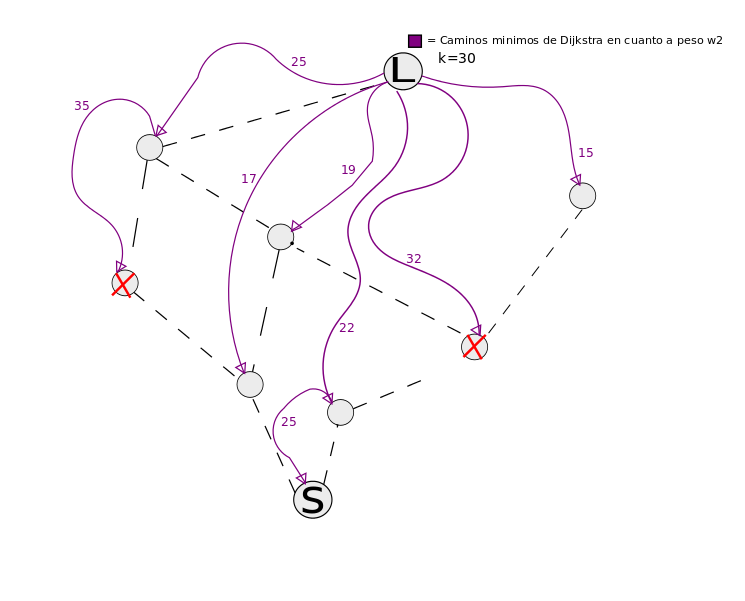
\includegraphics[scale=0.58]{img/inicializacion.png}
\end{center}	
\vspace{2mm}

Este dibujo representa la ejecuci\'on de la inicializaci\'on de la heur\'stica, donde el algoritmo de Dijkstra calcula los costos $w_1$ de los caminos m\'inimos de todos los nodos al nodo llegada (en violeta), y puede verse que aquellos nodos con caminos de costo mayor a $K$ ser\'an descartados.

\subsubsection{Heur\'istica golosa}

El algoritmo goloso en s\'i comparte su estructura con el algoritmo de Dijkstra sobre los costos $w_2$. El agregado al algoritmo es la estrategia previamente explicada, teniendo la informaci\'on que nos brindan $CostosW1$ y $CostoRecorrido$, cuando sacamos un nodo $v$ de la cola y procedemos a actualizar sus vecinos $x$, s\'olo vamos a considerar actualizar los valores $CostosW2$ y $precedesor$ para aquellos que sean factibles, es decir, aquellos para los cuales el costo $w_1$ del camino recorrido potencial recorrido hasta $v$ + el costo de la arista entre los nodos $(v,x)$ +  el costo $w_1$ del camino m\'inimo de $x$ a la llegada es menor o igual a K, dicho en t\'erminos del algoritmo: $costoRecorrido[v]+costo(v,x)+CostosW1[x]\leq K$. Esto nos asegura que el camino de un nodo nunca va a ser actualizado por un camino no factible.

\vspace{2mm}

La componente golosa del algoritmo, al igual que en el algoritmo de Dijkstra, es la elecci\'on en cada iteraci\'on del m\'inimo nodo de la cola de nodos.

\subsubsection{Pseudoc\'odigo}


\begin{algorithmic}[1]
\Statex

\Procedure{Heur\'istica Golosa}{grafo g, nodo u, nodo v, cota K}{ -$>$ camino}

\State $ vector<int> \: costosw_1[n] $
\State $vector<int> costosw_2[n]$
\State $vector<int> predecesores[n]$
\State $ vector<int> \: costoRecorrido[n] $
\State $camino \: c \gets [] $
\State $colaPrioridad \: cola \gets []$

\Statex

\State $ Dijkstra(g, v, costosw_1) $

\Statex

\For{$i\: from \: 0 \: to \: n-1$}
	\State $ costosw_2[i] \gets \infty $
	\State $ predecesores[i] \gets NULL $
	\State $ costoRecorrido[i] \gets 0 $	
\EndFor

\State $ costosw_2[u] \gets 0 $
\Statex
\State $ cola.push(costosw_2, u) $

\While{$cola != []$}
	\State $ par<costow_2, nodo> actual \gets cola.pop $
	\For{$ w \: : \: adyacentes(actual_2) $}
		\If{ $costoRecorrido[actual_2] + costow_1Arista(actual_2,w) + costosw_1(w)  \leq K $ }
		

			\If{$ costosw_2[w] > costosw_2[actual_2] + costow_2Arista(actual,w) $}
			\State $ costosw_2[w] \gets costosw_2[actual_2] + costow_2Arista(actual,w) $
			\State $ costoRecorrido[w] \gets costoRecorrido[actual_2] + costow_1Arista(actual_2,w) $
			\State $ predecesor[w] = actual $
			\State $cola.push(costow_2(w), w)$


			\EndIf

		\EndIf
	\EndFor

\EndWhile

\State $ c \gets reconstruirCamino(predecesor,v) $
\State $ return \:c $

\EndProcedure
\end{algorithmic}


\subsubsection{Complejidad}

El algoritmo comienza declarando vectores de longitud de tamano $n$, un camino de tamano $n^2$ y una cola de prioridad, en total tiempo $O(n^2)$. Acto seguido ejecuta el algoritmo de Dijkstra desde nodo llegada a todos los dem\'as, en tiempo $O((m+n)log n)$. Se ejecuta un ciclo que deja preparados los vectores a utilizar por el ciclo goloso, en $O(n)$ y dos asignaciones de tiempo constante.

\vspace{2mm}

El ciclo while va a iterar a lo sumo $n$ veces, ya que hay nodos no factibles que no ser\'an anadidos, y aquellos que si lo sos, son anadidos a lo sumo una \'unica vez (por la demostraci\'on de Dijkstra, al elegir el nodo con costo m\'inimo de la cola nos aseguramos que ese va a ser su costo m\'inimo y no va a ser necesario actualizarlo nuevamente). En cada iteraci\'on se obtiene y elimina el m\'inimo elemento de la cola en $O(logn)$. Nos queda analizar el ciclo $for$ interior, que para cada nodo itera sobre su lista de adyacentes. Como cada nodo es agregado una vez, entonces cada arista en la lista de cada nodo es examinada una vez durante el transcurso del algoritmo, por lo cual este ciclo for itera $m$ veces durante el transcurso del algoritmo. Dentro de este ciclo se realizan operaciones de tiempo constante excepto la operaci\'on $push$,la cual ejecuta en tiempo $O(logn)$, con lo cual el ciclo $for$ posee complejidad $O(mlogn)$.

\vspace{2mm}

Esto nos deja con una complejidad de: $O(n^2) + O((m+n)log n) + O(n log n) + O(n log m) = O(n^2 + m log n)$.

\vspace{2mm}

Usamos el tipo $set$ de la librer\'ia STL de c++, la cual nos asegura estas complejidades:
\begin{enumerate}
\item http://www.cplusplus.com/reference/set/set/
\item http://www.cplusplus.com/reference/set/set/begin/
\item http://www.cplusplus.com/reference/set/set/erase/
\end{enumerate}

\subsubsection{Soluci\'on Factible}

A continuaci\'on, vamos a demostrar que en caso de haber alg\'un camino factible desde la salida a la llegada (de costo $w_1$ total $\leq K$), la heur\'istica siempre va a encontrar un camino factible y por lo tanto, devolver una soluci\'on.

\vspace{2mm}

Consideremos el camino $C$, de costo $w_1$ m\'inimo del nodo de salida $u$ al nodo de llegada $v$. Supongamos que este existe y adem\'as su costo total es menor a la cota $K$. Supongamos que el algoritmo no puede encontrar un camino factible, y lleguemos a un absurdo. Tomemos a $x$, como el \'ultimo nodo $\in C$ para el cual el algoritmo puede actualizar sus valores, es decir, el \'ultimo nodo para el cual tuvo algu\'n vecino $a$ tal que $costoRecorrido[a] + costow_1Arista(a,x) + costosw_1(x)  \leq K $ y el algoritmo actualiz\'o valores. 

\vspace{2mm}

Sabemos que este nodo existe ya que existe $C$ un camino factible de costo m\'inimo $w_1$ $\leq K$ de $u$ a $v$, por lo tanto este nodo es al menos el segundo nodo de $C$, ya que sabemos que $costoRecorrido[u] + costow_1Arista(u,segundo) + costosw_1(segundo) \leq K $, al ser $costoRecorrido[u]=0$ y $costow_1Arista(u,segundo) + costosw_1(segundo)\leq K$ necesariamente ya que es un subcamino de $C$, y que el problema de camino m\'ino cumple el principio de optimalidad de Bellman, y el camino m\'inimo de $u$ a $v$ puede ser descompuesto como dos caminos $u-segundo$ y $segundo-v$ que a su vez son m\'inimos.

\vspace{2mm}

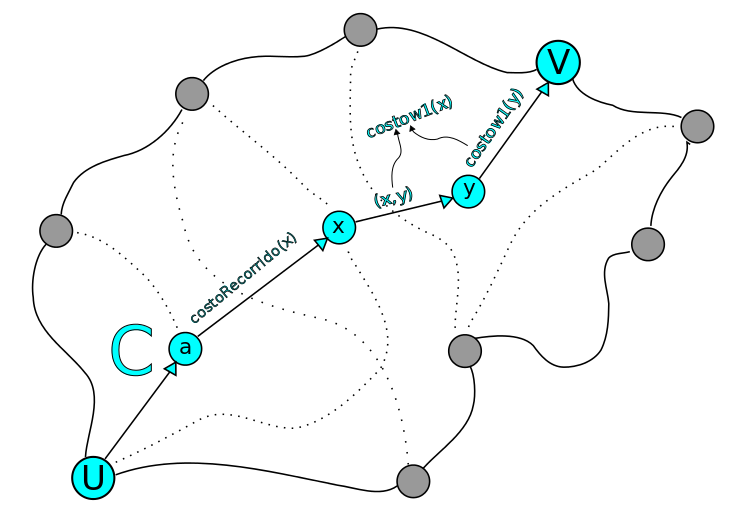
\includegraphics[scale=0.6]{img/caminoC.png}

Ahora consideremos el nodo siguiente del camino, llam\'emosle $y$. $y$ es el primer nodo del camino $C$ para el cual el algoritmo no puede actualizarlo ni insertarlo en la cola. Pero sabemos que $x$ es adyacente a $y$, y sabemos que para $x$, por haber sido actualizado por el algoritmo vale $costoRecorrido[x] + costosw_1(x) \leq K$. Y por no haber podido ser actualizado $y$ desde $x$, vale $costoRecorrido[x] + costow_1Arista(x,y) + costosw_1(y)  > K$. Pero esto nos deja en un absurdo, ya que $costosw_1(x)=  costow_1Arista(x,y) + costosw_1(y)$ exactamente, ya que ambos nodos forman parte de $C$, y por principio de optimalidad al sere $C$ el camino m\'inimo,  el camino m\'nimo de $x$ a la llegada va a ser el subcamino de $C$ de $x$ a la llegada, del cual forma parte $y$ y la arista entre $x$ e $y$.	

\vspace{2mm}

Llegamos a un absurdo al suponer que existe el camino $C$, y que el algoritmo en alg\'un punto para un nodo de $C$ no puede actualizarlo formando un camino factible. LLegamos a la conclusi\'on de que, o bien no existe ningu\'un camino factible en el grafo, o existe al menos uno y el algoritmo lo devuelve.

\subsection{Nivel de optimalidad de las soluciones}

Consideremos el siguiente grafo: $Origen=1, \:Destino = 3, \: K = 10$.

\begin{center}
	\includegraphics[scale=0.7]{img/{grafoBasicoMaloGreedy}.png}
\end{center}

\begin{lstlisting}[frame=single]
Salida golosa:
4 2 3 1 2 3
\end{lstlisting}

La salida de nuestro algoritmo nos devuelve el camino $1->2->3$ (para un $K$ no restrictivo), ya que la desici\'on golosa toma el m\'inimo de la cola en cada iteraci\'on y actualiza el nodo $3$ con el nodo $2$ ya que el camino $1->2$ (en rojo) tiene menos costo $w_2$ que la arista $(1,3)$ (en verde). Pero en este caso particular puede notarse como prima la desici\'on golosa en el algoritmo, sin tener en cuenta que este camino es mucho m\'as costoso en cuanto a $w_1$ que la arista. Si el grafo tuviese m\'as nodos adyacentes al nodo $3$, el haber elegido el camino va a restringir los caminos que va a poder tomar el algoritmo en las siguientes iteraciones. Por ejemplo, si el grafo fuese: $Origen=1, \:Destino = 6, \: K = 10$.

\begin{center}
	\includegraphics[scale=0.55]{img/{casoMaloGreedy}.png}
\end{center}

\begin{lstlisting}[frame=single]
Salida exacto:
10 5 4 1 3 4 6
\end{lstlisting}

\begin{lstlisting}[frame=single]
Salida golosa:
10 22 5 1 2 3 5 6 
\end{lstlisting}

Tenemos en color rojo la salida del algoritmo y en color verde el camino \'optimo. Vemos como la desici\'on golosa inicial restringi\'o claramente la elecci\'on de caminos posterior, forzando a tomar el camino mucho m\'as pesado que le permite llegar a destino sin superar la cota, el cual podemos hacerlo arbitrariamente m\'as costoso en cuanto a $w_2$ y alejar la soluci\'on de nuestro algoritmo de la \'optima tanto como queramos, aumentando los pesos $w_2$ o estirando el camino $3->5->6$ cuanto queramos (sin pasarnos de la cota $K$).

\subsection{Experimentacion: Mediciones de Performance}
En esta secci\'on se mostrar\'an resultados de complejidad temporal emp\'irica, veremos que los resultados coinciden razonablemente con el an\'alisis de complejidad te\'orica..
Para tener una mejor idea del comportamiento del algoritmo, realizamos pruebas sobre grafos aleatorios de distintos tama\~nos(en cantidad de nodos), y por cada cantidad $n$ de nodos, variamos las densidades de aristas dentro de cierto rango alrededor de una funcion de $n$, las densidades elegidas fueron:
\begin{itemize}
	\item m = $a*n + b$. Es decir una cantidad lineal de aristas en base a los nodos. $a \in \mathbb{N}_{>1}$
	\item m = $\frac{n*(n-1)}{2}$. Es decir grafos cercanos o iguales a cliques de n nodos.
\end{itemize}


\textbf{Nota: } Como mencionamos anteriormente, las funciones son variadas en un rango, es decir, por ejemplo, para el caso de cliques, los grafos generados tienen entre $\frac{n*(n-1)}{5}$ y $\frac{n*(n-1)}{2}$ aristas para aleatorizar mas la generacion de grafos densos.\\

\textbf{Nota: } Los graficos que contienen puntos rojos y una curva verde, indican, para cada valor del eje X(cantidad de nodos), los puntos rojos son los tiempos de ejecucion para los diferentes valores de aristas en el rango de la familia, asimismo, la curva verde indica el promedio de estos puntos para cada X. \\
\textbf{Nota: }Para verificar que se trata de una curva cuadratica dividimos las funciones por $n^1$, $n^2$, $n^3$, $n^4$ y como en los trabajos practicos anteriores concluimos de que curva se trata.\\

\subsubsection{Consideraciones acerca de la complejidad te\'orica}

En la secci\'on de anal\'isis de complejidad del algoritmo concluimos acotando la complejidad en $O(n^2 + m log n)$. Sin embargo, como informamos en la secci\'on anterior, nos vamos a limitar a dividir las funciones por potencias de $n$ de $1$ a $4$. Esto se debe a, adem\'as de una mayor simplicidad, a que en el caso de prueba con $m = a*n+b$, $m$ es lineal en cuanto a $n$, por lo tanto la complejidad se aproximar\'ia a $n^2 + nlogn$, con lo cual quedar\'a en el orden cuadr\'atico, y consideramos que va a bastar con considerarlo de este orden para realizar el an\'alisis de las divisiones. Por otro lado en el caso $m=n*(n-1)/a$, $m$ es cuadr\'atico en cuanto a $n$, y la complejidad se aproximar\'a a $n^2+n^2log n$, lo cual es del orden $O(n^2log n)$. Pero, considerando que como m\'aximo en nuestra experimentaci\'on usamos $n=2000$, $log(2000) \approx 11$, lo cual es casi despreciable, por lo cual tambi\'en consideraremos al algoritmo en el orden cuadr\'atico para realizar el an\'alisis.

\subsubsection{Rendimiento para grafos con densidad lineal de aristas}
\begin{itemize}
	\item cant nodos min = $50$
	\item cant nodos max = $2000$
	\item peso maximo w1 = $250$
	\item peso maximo w2 = $400$
	\item step nodos = $75$
	\item step aristas = $4500$
	\item aristas minimas = $n-1$
	\item aristas maximas = $10*n$
\end{itemize}

\begin{center}
	\textbf{Tiempo de ejecuci\'on en microsegundos para esta familia}\\
	\textbf{$y = f(x)$}\\
	\includegraphics[scale=0.7]{experimentos/golosa/golosa_lineal/{golosa.tmpplot_complexity_variation}.png}
\end{center}

\begin{center}
	\textbf{$y = f(x)/x$}\\
	\includegraphics[scale=0.7]{experimentos/golosa/golosa_lineal/{golosa.tmpplot_complexity_med_over_n}.png}
\end{center}

\begin{center}
	\textbf{$y = f(x)/x^2$}\\
	\includegraphics[scale=0.7]{experimentos/golosa/golosa_lineal/{golosa.tmpplot_complexity_med_over_n_square}.png}
\end{center}

\begin{center}
	\textbf{$y = f(x)/x^3$}\\
	\includegraphics[scale=0.7]{experimentos/golosa/golosa_lineal/{golosa.tmpplot_complexity_med_over_n_cube}.png}
\end{center}


\begin{center}
	\textbf{$y = f(x)/x^4$}\\
	\includegraphics[scale=0.7]{experimentos/golosa/golosa_lineal/{golosa.tmpplot_complexity_med_over_n_fourth}.png}
\end{center}


\subsubsection{Rendimiento para grafos con densidad cuadratica de aristas}
\begin{itemize}
	\item cant nodos min = $5$
	\item cant nodos max = $500$
	\item peso maximo w1 = $250$
	\item peso maximo w2 = $400$
	\item step nodos = $75$
	\item step aristas = $4500$
	\item aristas minimas = $\frac{n*(n-1)}{9}$
	\item aristas maximas = $\frac{n*(n-1)}{7}$
\end{itemize}								




\begin{center}
	\textbf{Tiempo de ejecuci\'on en microsegundos para esta familia}\\
	\textbf{$y = f(x)$}\\
	\includegraphics[scale=0.7]{experimentos/golosa/golosa_clique/{golosa.tmpplot_complexity_variation}.png}
\end{center}

\begin{center}
	\textbf{$y = f(x)/x$}\\
	\includegraphics[scale=0.7]{experimentos/golosa/golosa_clique/{golosa.tmpplot_complexity_med_over_n}.png}
\end{center}

\begin{center}
	\textbf{$y = f(x)/x^2$}\\
	\includegraphics[scale=0.7]{experimentos/golosa/golosa_clique/{golosa.tmpplot_complexity_med_over_n_square}.png}
\end{center}

\begin{center}
	\textbf{$y = f(x)/x^3$}\\
	\includegraphics[scale=0.7]{experimentos/golosa/golosa_clique/{golosa.tmpplot_complexity_med_over_n_cube}.png}
\end{center}


\begin{center}	
	\textbf{$y = f(x)/x^4$}\\
	\includegraphics[scale=0.7]{experimentos/golosa/golosa_clique/{golosa.tmpplot_complexity_med_over_n_fourth}.png}
\end{center}

\subsubsection{Conclusi\'on}

Como podemos ver en ambos casos, $f(x)$ es una funci\'on creciente, $f(x)/x$ tambi\'en es creciente, asemej\'andose a una curva lineal, y $f(x)/x^2$ deja de ser creciente para asemejarse a una constante en un intervalo entre $0.04 - 0.01$ en ambos casos. $f(x)/x^3$ y $f(x)/x^4$ dan como resultado valores muy cercanos al $0$, lo cual es el resultado de dividir una constante por la variable de experimentaci\'on (tiende a $0$).

\vspace{2mm}

Los experimentos nos dan indicios de complejidad cuadr\'atica, y esto se condice con la complejidad te\'orica $ O(n^2 + m log n) $ planteada acotada a grafos con $m$ lineal ($O(n^2)$) y cuadr\'atica ($O(n^2*logn)$ con $log(n)\approx 11$ como m\'aximo para $n=2000$).

\subsection{Experimentacion: Mediciones de Optimalidad de las soluciones obtenidas con esta heuristica}
En esta secci\'on nos vamos a dedicar al analisis de la calidad de las soluciones, es decir, dados conjuntos de grafos aleatorios, vamos a examinar el porcentaje de soluciones optimas obtenidas por esta heuristica y realizaremos algunos calculos estad\'isticos acerca de la lejan\'ia promedio de las soluciones obtenidas con respecto a la solucion exacta en los grafos del conjunto de instancias de las muestras. Para esto, se presentaran 2 experimentos, los cuales representan 2 densidades de grafos generados aleatoriamente.\\
\textbf{Nota: }La lejan\'ia entre 2 soluciones se mide haciendo el siguiente calculo: 
$ 100 *(\frac{solucionHeuristica}{solucionOptima} - 1)  $\\
\textbf{Nota: } Los calculos estadisticos (promedio y desviacion estandar) se realizan sobre la lista de resultados obtenida de la ejecucion secuencial y el calculo de la lejania mencionado aqui arriba para cada uno de los algoritmos(exacto y heuristica) sobre cada instancia del conjunto de pruebas.

\subsubsection{Grafos aleatorios de baja densidad de aristas}
\textbf{Parametros del experimento:}
\begin{itemize}
	\item Cantidad de grafos analizados: 25
	\item Cantidad minima de nodos: 100
	\item Cantidad maxima de nodos: 2200
	\item Rango peso $w_1$: [0..250]
	\item Rango peso $w_2$: [0..400]
	\item Cota de $w_1$: 200
	\item Cantidad minima de aristas: $n-1$
	\item Cantidad maxima de aristas: $10*n$
\end{itemize}

\textbf{Resultados del analisis:}
\begin{lstlisting}[frame=single]
	Heuristica da la solucion optima: 100.0% de los casos
	Lejania promedio de la heuristica a la solucion optima: 0%
	Desv. estandar de la lejania entre las soluciones: 0
	Minima lejania entre bqlocal y exacta: 0
	Maxima lejania entre bqlocal y exacta: 0
\end{lstlisting}

Realmente podemos observar una efectividad impecable para grafos de baja densidad. La heur\'istica golosa resulto ser excelente para casi todos los casos de poca densidad(tengamos en cuenta que esto es un muestreo de grafos, no representan todos los grafos de baja densidad.)

\subsubsection{Grafos aleatorios de alta densidad de aristas}
\textbf{Parametros del experimento:}
\begin{itemize}
	\item Cantidad de grafos analizados: 48
	\item Cantidad minima de nodos: 10
	\item Cantidad maxima de nodos: 300
	\item Rango peso $w_1$: [0..250]
	\item Rango peso $w_2$: [0..400]
	\item Cota de $w_1$: 200
	\item Cantidad minima de aristas: $\frac{n * (n-1)}{3}$
	\item Cantidad maxima de aristas: $\frac{n * (n-1)}{2}$
\end{itemize}

\textbf{Resultados del analisis:}
\begin{lstlisting}[frame=single]
	Heuristica da la solucion optima: 79.166% de los casos
	Lejania promedio de la heuristica a la solucion optima: 14.622 %
	Desv. estandar de la lejania entre las soluciones: 63.0996
	Minima lejania entre bqlocal y exacta: 0
	Maxima lejania entre bqlocal y exacta: 433.300%
\end{lstlisting}

Para grafos de alta densidad, ya la heur\'istica comienza a fallar, pero de forma relativamente leve, solo en un 20.833\% de los casos, consideramos que un 14.622\% de lejania en las soluciones provistas por la heuristica respecto a la soluci\'on \'optima ser\'ia aceptable en algunas aplicaciones que no requieran una soluci\'on estrictamente optima dada la mejora en tiempo que se obtiene utilizando la heur\'istica.(Recordemos que la soluci\'on exacta implementada tiene complejidad no polinomial). Con respecto a la desviaci\'on estandar y la m\'axima lejan\'ia podemos ver que hay casos donde la soluc\'ion se aleja bastante, un 433\% del optimo, pero dada la desviaci\'on de 63.0996 vemos que no es algo que ocurra en forma general.

Como conclusi\'on pensamos que es una heur\'istica bastante bien lograda dados estos valores de optimalidad y su complejidad temporal.